% Safe, Self-Evolving, and Swift Coding Agent (S-Code)
% A coding agent's editor, surrounded by its three properties: safe, self-evolving, swift.
\documentclass[tikz,border=0pt]{standalone}
% Shared look for the TikZ publication thumbnails.
% Canvas: 16cm x 10cm (16:10, matching the 640x400 WebP output), white, site palette.
% Labels are large (\lbl) because thumbnails are shown about 200px wide.
\usepackage[T1]{fontenc}
\usepackage{helvet}
\renewcommand{\familydefault}{\sfdefault}
\usepackage{amsmath,amssymb}
\usepackage{fontawesome5}
\usetikzlibrary{arrows.meta,calc,positioning,shapes.geometric,shapes.callouts,decorations.pathmorphing,shadows}

\definecolor{ink}{HTML}{2B2D42}
\definecolor{accent}{HTML}{B509AC}
\definecolor{teal}{HTML}{1E9BC0}
\definecolor{violet}{HTML}{6C5CE7}
\definecolor{orange}{HTML}{F28C28}
\definecolor{sun}{HTML}{F2C14E}
\definecolor{leaf}{HTML}{2CA58D}
\definecolor{alert}{HTML}{E5484D}
\definecolor{mist}{HTML}{EEF0F5}

\tikzset{
  every picture/.append style={line cap=round, line join=round},
  card/.style={rounded corners=10pt, draw=#1!75!black, line width=1.4pt, fill=#1!12},
  arrow/.style={-{Stealth[length=10pt,width=9pt]}, line width=2.2pt, draw=#1},
  soft shadow/.style={drop shadow={shadow xshift=0pt, shadow yshift=-3pt, opacity=0.18, fill=ink}},
  badge/.style={circle, fill=#1!14, draw=#1, line width=2pt, minimum size=2.3cm, text=#1},
}
\newcommand{\thumbcanvas}{\useasboundingbox[fill=white] (0,0) rectangle (16,10);}
\newcommand{\lbl}[1]{{\fontsize{20}{22}\selectfont\bfseries #1}}
\newcommand{\icon}[2][34]{{\fontsize{#1}{#1}\selectfont\faIcon{#2}}}
% Window chrome: dark editor panel with traffic-light dots. Args: x0, y0, x1, y1.
\newcommand{\editor}[4]{%
  \fill[ink, rounded corners=12pt, soft shadow] (#1,#2) rectangle (#3,#4);
  \foreach \c [count=\k] in {alert,sun,leaf} \fill[\c] ({#1+0.15+0.42*\k},{#4-0.42}) circle (0.13);
}

\newcommand{\slbl}[1]{{\fontsize{17}{19}\selectfont\bfseries #1}}
\begin{document}
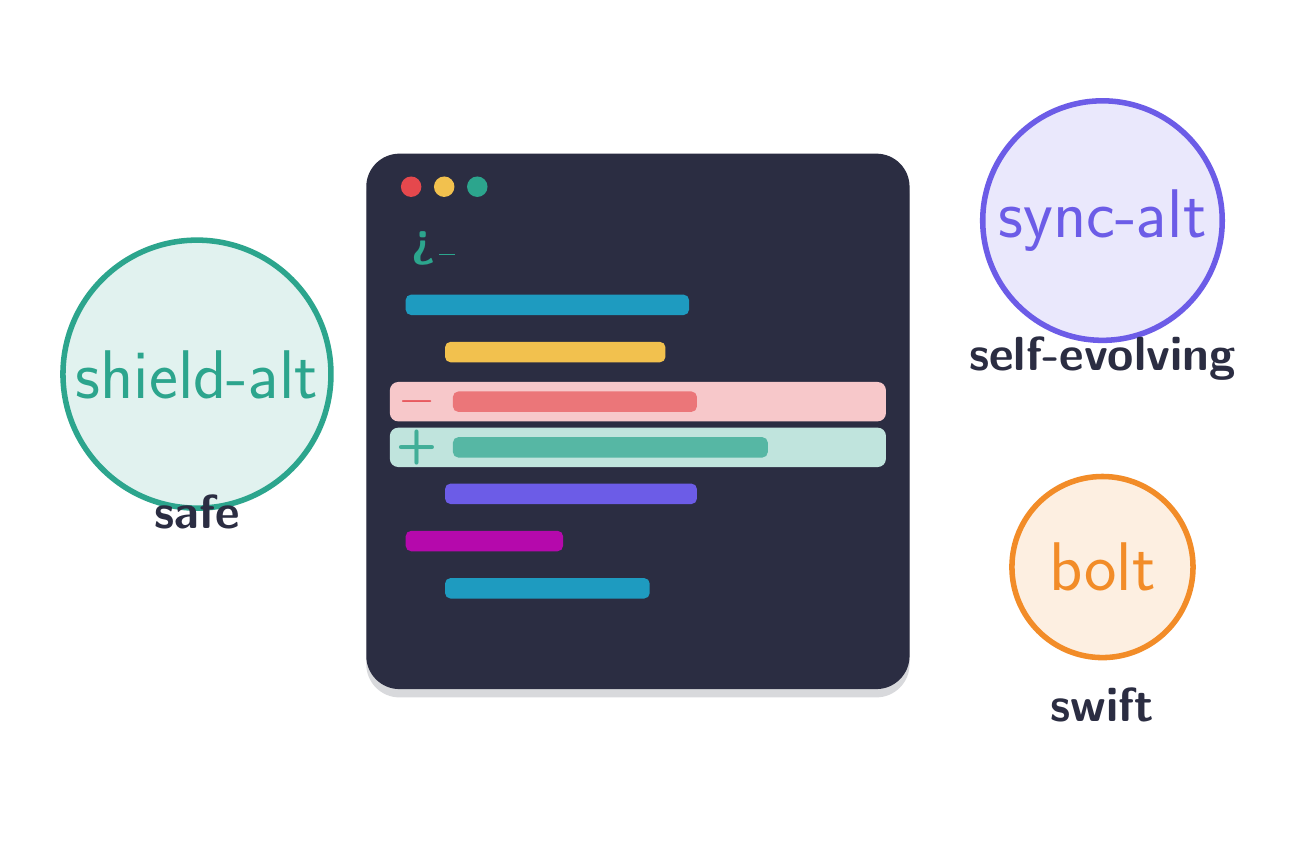
\begin{tikzpicture}
\thumbcanvas
\editor{4.3}{1.6}{11.2}{8.4}
\node[text=leaf, anchor=west] at (4.75,7.2) {\slbl{>\_}};
\foreach \y/\x/\w/\c in {6.35/4.8/3.6/teal,5.75/5.3/2.8/sun,3.95/5.3/3.2/violet,3.35/4.8/2.0/accent,2.75/5.3/2.6/teal}
  \fill[\c, rounded corners=2pt] (\x,\y) rectangle ++(\w,0.26);
% A self-applied diff.
\fill[alert!30, rounded corners=3pt] (4.6,5.0) rectangle (10.9,5.5);
\node[text=alert!90!white] at (4.95,5.25) {\slbl{$-$}};
\fill[alert!75, rounded corners=2pt] (5.4,5.12) rectangle ++(3.1,0.26);
\fill[leaf!30, rounded corners=3pt] (4.6,4.42) rectangle (10.9,4.92);
\node[text=leaf!90!white] at (4.95,4.67) {\slbl{+}};
\fill[leaf!80, rounded corners=2pt] (5.4,4.54) rectangle ++(4.0,0.26);
% Properties.
\node[badge=leaf] at (2.15,5.6) {\icon{shield-alt}};
\node[text=ink] at (2.15,3.85) {\slbl{safe}};
\node[badge=violet] at (13.65,7.55) {\icon{sync-alt}};
\node[text=ink] at (13.65,5.8) {\slbl{self-evolving}};
\node[badge=orange] at (13.65,3.15) {\icon{bolt}};
\node[text=ink] at (13.65,1.4) {\slbl{swift}};
\end{tikzpicture}
\end{document}
